\section{Non-parametric classification}

\subsection{The setting}

\begin{frame}\frametitle{\subsecname for M-way classification}

\mode<article>{
Specifying the data and model for a multi-class classification with $M$ classes (i.e. $M$-way classification)
}

\begin{itemize}
	\item \underline{Data}:\\

	\begin{equation*}
	\Big\{ \left(\vec x^{(\alpha)}, \vec y^{(\alpha)}_{T} \right) \Big\}\,
	\end{equation*}

	where 
	\begin{itemize}
	\item[] $\alpha = 1,\ldots,p$ and
	\item[]$\vec y_T^{(\alpha)} \in \{0, 1\}^M$ with $\sum_{c=1}^{M} (y_{T})_c = 1$ (one-hot encoding of class labels),
	\end{itemize}

	\pause

	\item \underline{Model}:\\

	\begin{equation*}
	\vec y(\vec x) \in \R^M 
	\end{equation*}
	with 
	\begin{itemize}
	\item[] $\sum_{c=1}^{M} y_c(\vec x) = 1$ and
	\item[] $y_c(\vec x)\,\ge\,0\; \forall c$
	\end{itemize}
	
	Use $\vec y(\vec x)$ to give
	\begin{itemize}
	\item probabilities of the predicted class (e.g. $y_5(\vec x) = 0.75\; \leadsto$ class ``5'' with 75\% probability.
	\item hard predictions/decisions: $\argmax_{c=1,\ldots,M} y_c(\vec x)$
	\end{itemize}

\end{itemize}

\end{frame}

\subsection{k nearest neighbor}


\begin{frame}\frametitle{\subsecname}

Prediction follows the majority vote of the $k$ nearest neighbors around the query point.

\begin{figure}[ht]
     \centering
	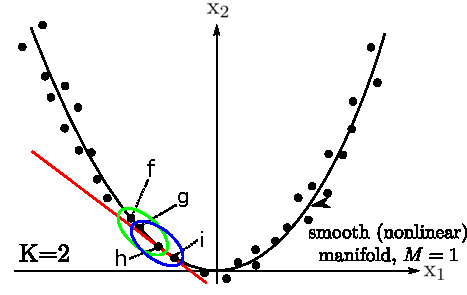
\includegraphics[width=0.2\textwidth]{img/section4_fig11_K2}
     \mode<article>{
	\caption{Basic RNN architecture}
	}
	\label{fig:rnn} 
\end{figure}

\end{frame}

\begin{frame}\frametitle{\subsecname}

Let $k$NN$(\vec x)$ be the indices $\{\alpha_1, \alpha_2,\ldots,\alpha_k\}$ of the $k$ data points closest to $\vec x$ w.r.t. Euclidean norm:

\begin{equation}
\alpha_j = \argmin_{\alpha \in \{1,\ldots,\p\} }
\end{equaiton}

\end{frame}
